\begin{apendicesenv}
\partapendices

\chapter{Proposta de uma estratégia CA fragmentada para Camphs1D}

A estratégia CA fragmentada proposta neste trabalho, para o sistema CA Camphs1D, tem como objetivo de subdividir o domínio em blocos menores, processados em um \textit{loop}, através de um CORE CA implementado em hardware. Sendo assim, a implementação do CORE CA pode ter uma quantidade bem reduzida de células autônomas, pois o este CORE será reutilizado até o processamento de todas as células autômatas do domínio considerado.

O termo ``fragmentada'' também faz alusão ao fato de que, no interior do CORE CA, as células autômatas não estão conectadas entre si. Temos apenas um aglomerado de células autômatas, capazes de operar, simultaneamente, os sinais de entrada do CORE CA. Em outras palavras, o CORE CA deve possui um barramento de dados capaz de enviar as informações que, outrora, seriam recebidas por estas células caso elas estivessem posicionadas, e integradas, dentro do domínio completo. De maneira semelhante, nas saídas do deste CORE CA temos os mesmos sinais que, outrora, deveriam ser repassados para as suas células vizinhas, caso as mesnas estivessem conectadas no domínio completo.     

Percebe-se que temos uma inversão de funções. No caso da estratégia completa (adotada nas implementações deste trabalho) as células autônomas estão integradas em hardware, respeitando a geometria considerada. Por este motivo, não precisamos nos preocupar, em nível de software, com a integração dos sinais processados. No caso da estratégia fragmentada, os sinais processados estão integrados através de um algoritmo descrito em software e, portanto, não precisamos nos preocupar com a integração celular, em nível de hardware.

A seguir será apresentada a solução CA fragmentada do mesmo problema atacado pelo organismo artificial Camphs1DB9G2. Para esta solução, foi desenhado um CORE CA com apenas 5 células autônomas, capazes de resolver o domínio de 185 células proposto. Para efeito de uma melhor prototipação do circuito, foi utilizado um paradigma de programação orientada a objeto (POO). Todos os artefatos deste projeto estão apresentados a seguir.

\begin{figure}
	\centering
	\label{frag.png}
		\includegraphics[keepaspectratio=true,scale=0.8]{figuras/DiagramaClassesFragmentada.drawio.png}
	\caption{\label{fig:fragmentada_classes}Mapa de classes utilizado na solução fragmentada operada por Camphs1DH1G4.}
\end{figure}

Na Figura \ref{fig:fragmentada_classes} temos o diagrama de classes implementado na solução fragmentada proposta. Nesta estratégia, o organismo artificial denominado Camphs1DH1G4, composto por 1 célula autômata do tipo HCA1D e 4 células autômatas do tipo GCA1D, deverá ser capaz de operar todas as interações celulares realizadas pelo organismo Camphs1DB9G2, em sua forma integral. 

O paradigma POO nos permite visualizar a solução em software de uma maneira maneira mais próxima da realidade do circuito, pois temos o benefício do encapsulamento de informações, variáveis, funções e demais tratamentos de sinais. Seguindo este pensamento, os objetos representam os componentes que devem se interagir no circuito, operando os sinais envolvidos. 

\begin{figure}
	\centering
	\label{frag.png}
		\includegraphics[keepaspectratio=true,scale=0.7]{figuras/Untitled Diagram.drawio.Funcoes.png}
	\caption{\label{fig:fragmentada_funcoes}Mapa de classes utilizado na solução fragmentada operada por Camphs1DH1G4.}
\end{figure}

A estratégia fragmentada está apresentada, de maneira simplificada, na Figura \ref{fig:fragmentada_funcoes}. Temos três estágios de operação, um para cada configuração de fonte. Em cada estágio, para cada ciclo de relógio, o componente Camphs1DH1G4 percorre o vetor de memória processando os sinais, entre as células autômatas, como se suas células estivessem realmente naquelas posições. O resultado é imediatamente armazenado em outro vetor de memória, que tem o papel de guardar o estado presente. Após a varredura, o vetor de memória presente transfere seus valores para o vetor de memória passado, e um novo ciclo de relógio se inicia. 

Temos, nesta simulação, 187 células autômatas ``abstratas'' sendo operadas por apenas 5 células ``reais''. A solução fragmentada apresentou a mesma solução do modelo de referência, adotada para validação do organismo artificial Camphs1DB9G2. Por outro lado, o organismo Camphs1DH1G4 necessitou de 46 operações para realizar o trabalho que o organismo Camphs1DB9G2 executa a cada ciclo de relógio. 

\chapter{Modeling wave propagation using cellular automata on Chip}

O trabalho intitulado \textit{Modeling wave propagation using cellular automata on Chip} foi publicado no \textit{ $34^{th}$ Symposium on Integrated Circuits and Systems Design} (SBCCI 2021). O mesmo pode ser apreciado nas páginas seguintes. 

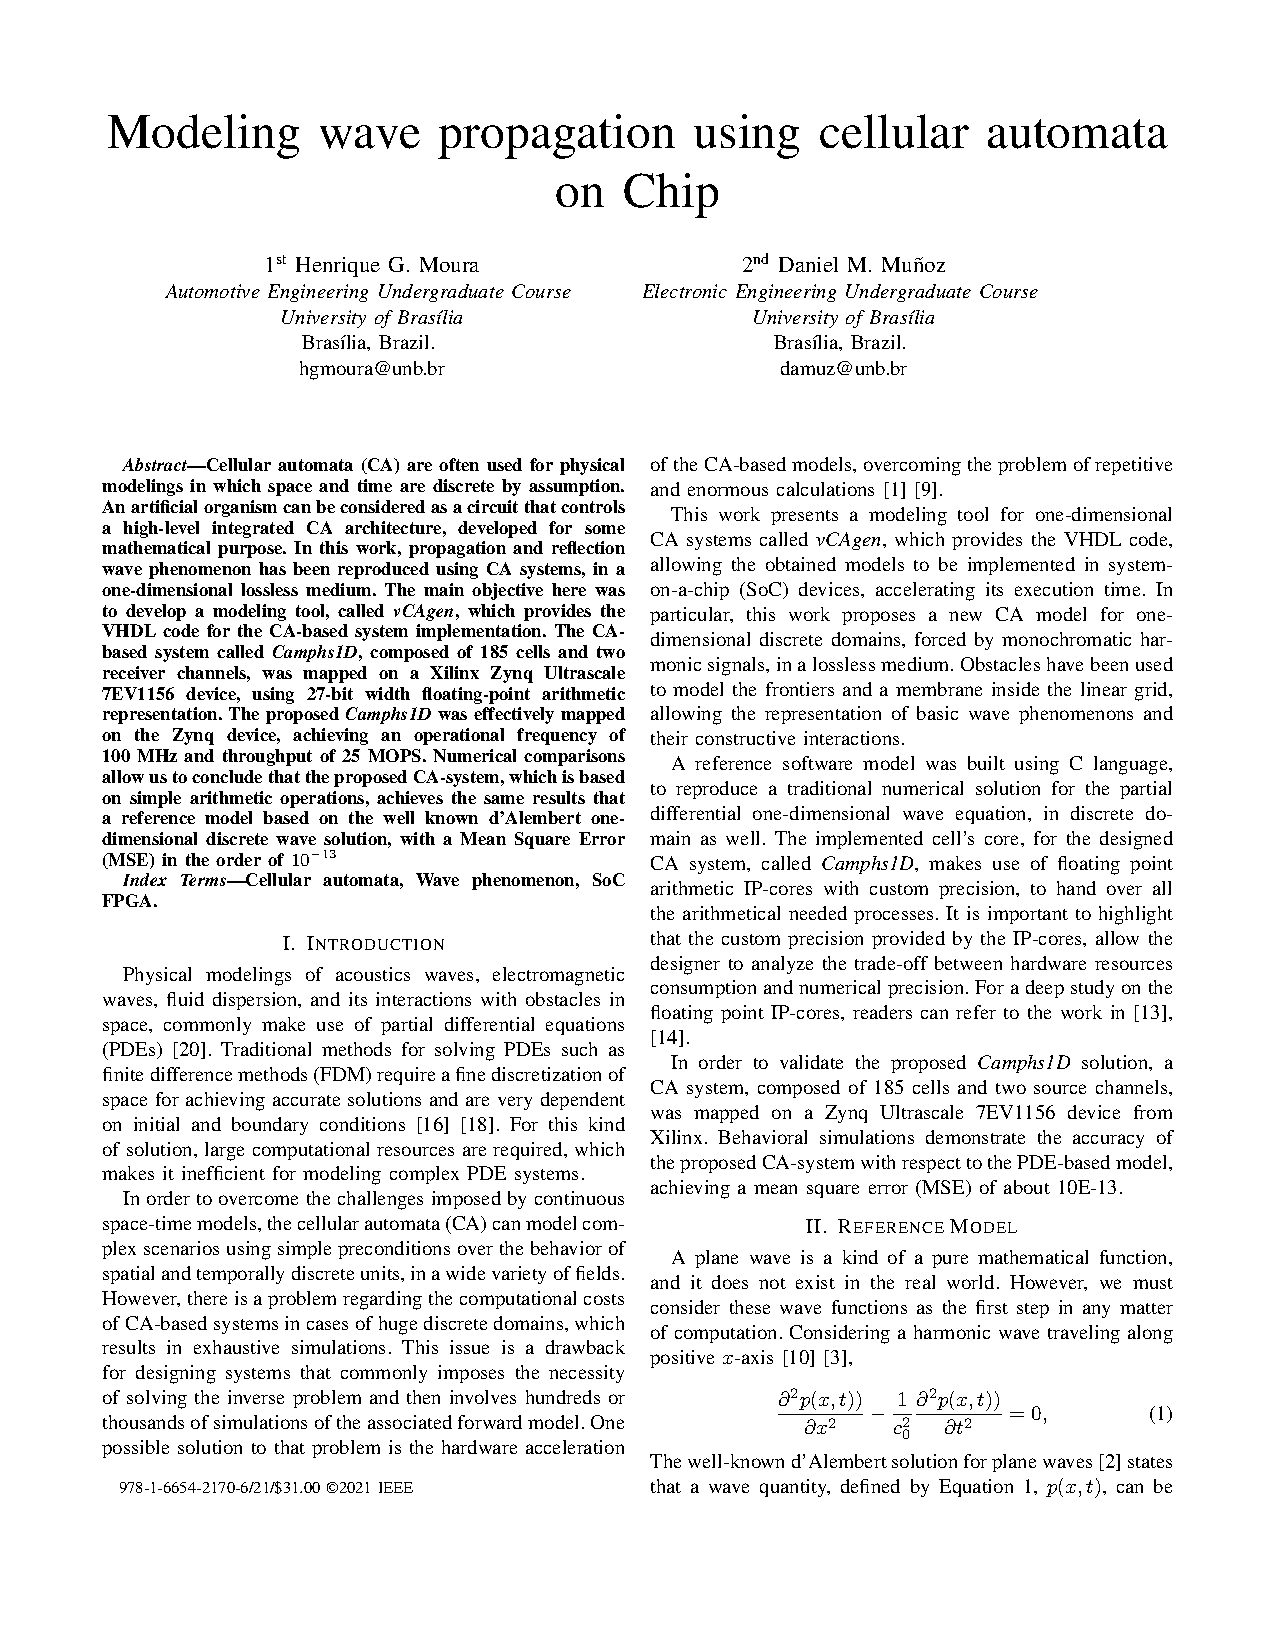
\includepdf[pages=-]{fixos/artigo.pdf}

\end{apendicesenv}